\thispagestyle{plain}
\begin{center}
  \begin{figure}[h]
    \centering
    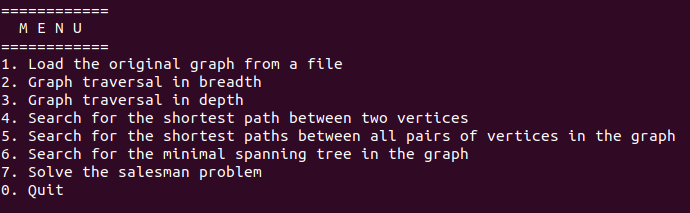
\includegraphics[scale=0.7]{1.png}
    \caption{GUI}
  \end{figure}
  Console interface of the program.\\

  \begin{figure}[h]
    \centering
    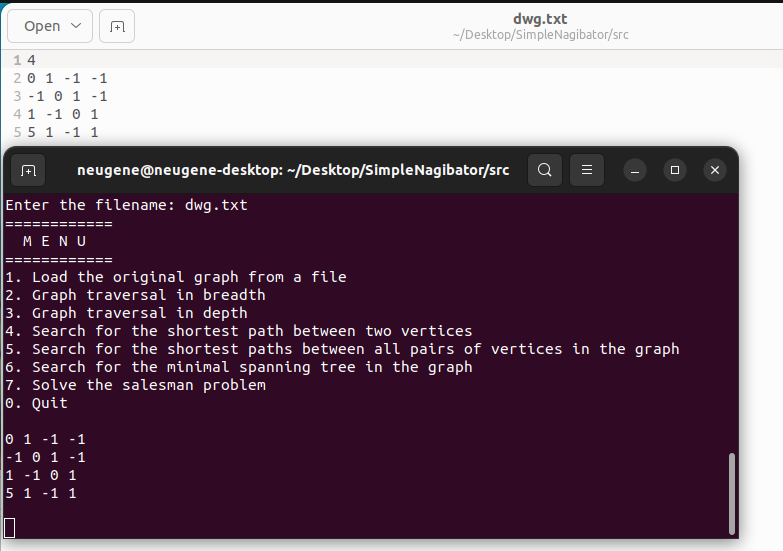
\includegraphics[scale=0.45]{2.png}
    \caption{1st menu item}
  \end{figure}
  Loading a graph from a file in adjacency matrix format.\\

\newpage

  \begin{figure}[h]
    \centering
    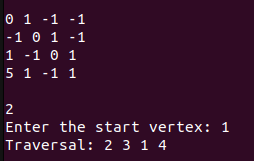
\includegraphics[scale=1]{3.png}
    \caption{2nd menu item}
  \end{figure}
  Breadth-first search in the graph from a given vertex.\\

  \begin{figure}[h]
    \centering
    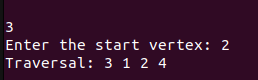
\includegraphics[scale=1]{4.png}
    \caption{3rd menu item}
  \end{figure}
  A non-recursive depth-first search in the graph from a given vertex.\\

  \begin{figure}[h]
    \centering
    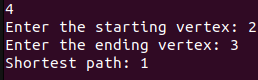
\includegraphics[scale=1]{5.png}
    \caption{4th menu item}
  \end{figure}
  Searching for the shortest path between two vertices in a graph using Dijkstra's algorithm.\\

  \newpage

  \begin{figure}[h]
    \centering
    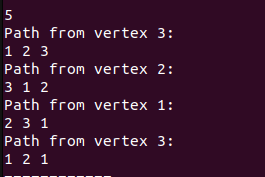
\includegraphics[scale=1]{6.png}
    \caption{5th menu item}
  \end{figure}
  Searching for the shortest paths between all pairs of vertices in a graph using the Floyd-Warshall algorithm.\\

  \begin{figure}[h]
    \centering
    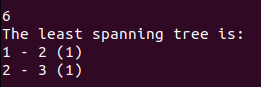
\includegraphics[scale=1]{7.png}
    \caption{6th menu item}
  \end{figure}
  Searching for the minimal spanning tree in a graph using Prim's algorithm.\\

  \begin{figure}[h]
    \centering
    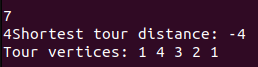
\includegraphics[scale=1]{8.png}
    \caption{7th menu item}
  \end{figure}
  Solving the traveling salesman's problem using the ant colony algorithm.\\
\end{center}

